\section{Infrastructure}
\label{sec:rel}
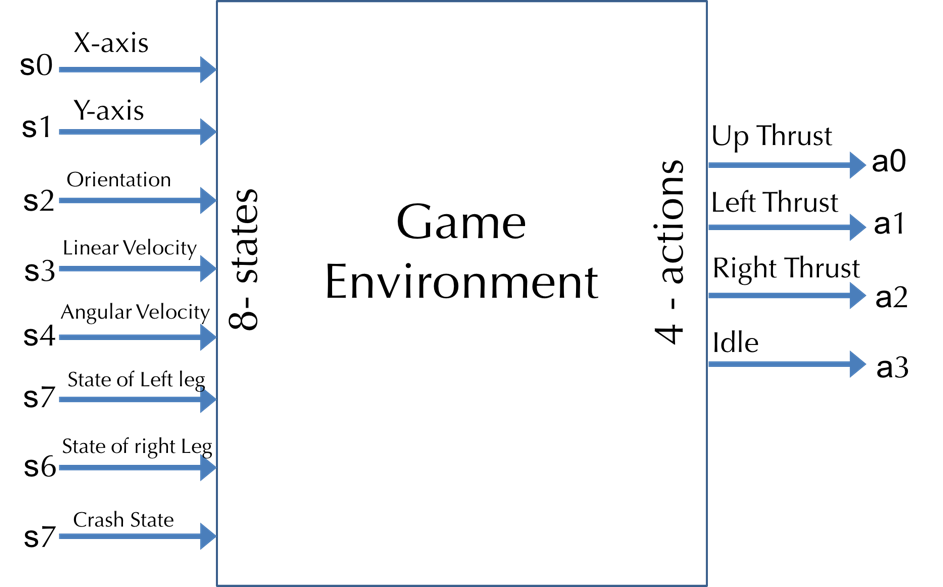
\includegraphics[scale=1.0,width=1.0\columnwidth]{figures/game_env.png}%
\newline
We have used the OpenAI gym library to train our agent. Although some insights are provided in Box2D Lunar Lander on the OpenAI website, thorough exploration of actions, state space, environment etc. was done before starting to solve the problem. Following is the description:

\subsection{Actions}
In this game, four discrete actions are available to the playing agent at any time frame: 

\begin{enumerate}[label=(\alph*)]
\item Do nothing
\item Fire left orientation engine (rotates the lunar lander clockwise)
\item Fire main engine (provides upward thrust)
\item Fire right orientation engine (rotates the lunar lander anti-clockwise)
\end{enumerate}

The agent can choose only one action among the given actions at a given time frame.

\subsection{Terrain} 
The terrain is a combination of 10 points, and the helipad(landing zone) is fixed between 5th and 6th points towards the center. The values of the height of the landing zone(5th and 6th points on the terrain) are viewport height divided by 4, and the rest of the points are randomly sampled between 0 to H/2 using \textit{numpy} random and smoothened (averaging 3 continuous points).

\subsection{Initial State}

The state is 8 dimensional values of different parameters of the lunar lander at any given time. The starting state is randomly initialized (the lunar lander takes a step in the world through the "idle" action) with certain bounds based on the environment.

Inspecting code of open\_ai lunar lander, we see that the initial states are defined by simulating the environment in one frame (calling box world simulation using time step as $1/FPS$). Using this simulation, elaborating the initial state as follows:

\begin{enumerate}
\item Position X (Initial Position X: final x which changed from half of viewport width to a value after taking "idle" action before the simulation)
\item Position Y (Initial Position Y: final y which changed from from the viewport height to a value after taking "idle" action before simulation)
\item Velocity X (Initial Velocity X: final velocity x changed from 0 to a value after taking "idle" action before simulation)
\item Velocity Y (Initial Velocity Y: final velocity y which changed from 0 to a value after taking "idle" action before simulation)
\item Current lander angle (Initial lander angle: final lander angle after simulation on "idle" action from 0 degrees)
\item Angular velocity (Initial angular velocity: final angular velocity after simulation on "idle" action from 0 angular velocity)
\item Left leg contacted the surface (Initial value: False, since there's is no probability that the lunar lander's leg will touch the moon surface when at the top)
\item Right leg contacted the surface (Initial value: False)
\end{enumerate}

\subsection{End State}

The episode ends in the following scenarios:

\begin{enumerate}
\item  When the lunar lander goes outside of the viewport bounds, the game is over with -100 is negative reward.
\item  When the lunar lander touches the ground with a high velocity
\item When the lunar lander touches the ground with body part except the legs
\item When the lunar lander stabilises on the moon's surface (change in shape of lunar lander is constantly 0 for a number of frames)
\end{enumerate}

\subsection{Rewards and Transitions}

Before defining the rewards, let's define the shape of the lunar lander which decides the rewards. The shape of the lunar lander is a function of position coordinates $(x, y)$, linear velocities $(v_x, v_y)$, lander angle $\theta$ and contact of both the lander legs. We are interested in finding the change of shape at every step for the lunar lander to calculate the rewards for each given action. Shape change is given by subtraction of previous shape and current shape. Formally, shaping at time frame $t$:

\begin{align*}
\text{shaping}_{t} = &- 100*(x^2 + y^2) \\
           & - 100*(v_x^2 + v_y^2) \\
            &- 100*abs(\theta) + 10*(\text{Left leg contacted}) + 10*(\text{Right leg contacted}) \\
\text{shape change} = & \text{shaping}_t - \text{shaping}_{t-1}
\end{align*}

The rewards are defined as follows:

\begin{enumerate}
\item If the lunar lander crashes, or goes out of the bounds: $-100$
\item If the lunar lander is not awake anymore (stabilises at 0 shape change): $+100$
\item Doing nothing: shape change 
\item Firing the engine: shape change - 0.3
\item Rotating: shape change - 0.03
\end{enumerate}

The total reward will automatically be a sum of all the rewards at each time frame, and if the lander touches the ground with it's legs, will add those rewards to the total rewards earned during an episode. Transition probabilities are unknown, we get next states by simulating the lunar lander in the box environment given the current state and action taken. \\

\textbf{Note}: The transition probabilities and rewards are unknown to our agent, which it will try to figure out through exploration and incorporate in learning. 

